\documentclass[headings=optiontoheadandtoc,listof=totoc,parskip=full]{scrartcl}

\usepackage[tbtags]{amsmath,mathtools}
\usepackage{amssymb}
\usepackage{enumitem}
\usepackage[margin=.75in]{geometry}
\usepackage[headsepline]{scrlayer-scrpage}
\usepackage[USenglish]{babel}
\usepackage{hyperref}
\usepackage{graphicx}
\usepackage{float}
\usepackage{physics}
\usepackage[format=hang, justification=justified]{caption}
\usepackage{xcolor}
\usepackage{mathbbol}

\usepackage{cleveref} % Needs to be loaded last

\hypersetup{
	linktoc = all,
	pdfborder = {0 0 .5 [ 1 3 ]}
}

\def \reals {\mathbb{R}}
\DeclareMathOperator*{\argmax}{arg\,max}
\DeclarePairedDelimiter\floor{\lfloor}{\rfloor}

\pagestyle{scrheadings}
\rohead{Khedekar, Mangat \& Novotny}
\lohead{CS 479 Programming Assignment 3}

\title{Programming Assignment 3}
\subtitle{CS 479\\\url{https://github.com/alexander-novo/CS479-PA3}}
\author{Nikhil Khedekar\\33\%\\\Cref{sec:part-3} \and Mehar Mangat\\33\%\\\Cref{sec:part-3} \and Alexander Novotny\\33\%\\\Cref{sec:part-1}}
\date{Due: April 26, 2021 \\ Submitted: \today}

\begin{document}
\maketitle
\tableofcontents
\pagenumbering{gobble}

\newpage
\pagenumbering{arabic}

%%%%%%%%%%%%%%%%%%%%%%

\section{Theory}

This assignment considers the usage of Principal Component Analysis for dimensionality reduction for a dataset of images for the purpose of face recognition. 

\subsubsection{Principal Component Analysis (PCA)}
Principal Component Analysis (PCA) is a method for reducing the dimensionality of high dimensional data while preserving as much information as possible. The way this works is by the projection of the sample data along its principal distribution directions. Intuitively, this can be understood by finding the directions that capture the highest variance of the data and projecting the data along these directions as seen for a 2D to 1D case in. 


For some given sample data $\mathbf{X} = \{\vec x_i \in \reals^N, 1 \leq i \leq M\}$, where $M$ is the number of samples in the data set, the sample covariance matrix $\Sigma_x$ can be found using \cref{eq:mean} and \cref{eq:cov_mat}, where $\Bar{x}$ is the sample mean and $\Phi_i$ are the normalized data points:

\begin{equation} \label{eq:mean}
    \mathbf{\Bar{x}} = \frac{1}{M}\sum_{i = 1}^{M}\mathbf{x}_i
\end{equation}

\begin{equation}
    \mathbf{\Phi_i} = \mathbf{x}_i - \mathbf{\Bar{x}}
\end{equation}

\begin{equation} \label{eq:cov_mat}
    \mathbf{\Sigma_x} = \frac{1}{M}\sum_{i = 1}^M(\mathbf{x} - \mathbf{\Bar{x}})(\mathbf{x} - \mathbf{\Bar{x}})^T = \frac{1}{M}\sum_{i = 1}^{M}\mathbf{\Phi}_i\mathbf{\Phi}_i^T 
\end{equation}

\Cref{eq:cov_mat} can be further simplified to \cref{eq:cov_mat_simp} using \cref{eq:a_mat}.

\begin{equation}\label{eq:cov_mat_simp}
    \mathbf{\Sigma_x} = \frac{1}{M}\mathbf{A}\mathbf{A}^T
\end{equation}

\begin{equation}\label{eq:a_mat}
    \mathbf{A} = [\Phi_1 \Phi_2 ... \Phi_M]    
\end{equation}

The eigenvectors and eigenvalues of the covariance matrix have the special property that the eigenvectors form an orthogonal basis in $R^N$ for the sample data with the corresponding eigenvalues representing the variance of the data in these directions. The eigenvectors and corresponding eigenvalues are obtained using \cref{eq:eigenvec_and_eigenval}.

\begin{equation}\label{eq:eigenvec_and_eigenval}
    \mathbf{\Sigma_x}\mathbf{u_i} = \lambda_iu_i
\end{equation}

In our notation, we assume that the eigenvalues are indexed in descending order, namely, $\lambda_1 > \lambda_2 > ... > \lambda_N$. Using the eigenvectors as the new basis we can represent our data samples $\mathbf{x} \in \reals^N$ as:

\begin{equation}
    test
\end{equation}

\subsubsection{Eigenfaces and Facial Recognition}

The first widely successful method of solving the facial recognition problem is the eigenface method. An eigenface


\section{Implementation}
\section{Results and Discussion}

\begin{figure}[H]
	\centering
	\includegraphics[width=.4\textwidth]{../out/mean-H} \quad
	\includegraphics[width=.4\textwidth]{../out/mean-L}
	\caption{The sample mean face for the high resolution data set and the low resolution data set, respectiely.}
\end{figure}

\begin{figure}[H]
	\centering
	\includegraphics[width=.09\textwidth]{../out/eigenface-H-largest-1}
	\includegraphics[width=.09\textwidth]{../out/eigenface-H-largest-2}
	\includegraphics[width=.09\textwidth]{../out/eigenface-H-largest-3}
	\includegraphics[width=.09\textwidth]{../out/eigenface-H-largest-4}
	\includegraphics[width=.09\textwidth]{../out/eigenface-H-largest-5}
	\includegraphics[width=.09\textwidth]{../out/eigenface-H-largest-6}
	\includegraphics[width=.09\textwidth]{../out/eigenface-H-largest-7}
	\includegraphics[width=.09\textwidth]{../out/eigenface-H-largest-8}
	\includegraphics[width=.09\textwidth]{../out/eigenface-H-largest-9}
	\includegraphics[width=.09\textwidth]{../out/eigenface-H-largest-10}\\
	\includegraphics[width=.09\textwidth]{../out/eigenface-H-smallest-1}
	\includegraphics[width=.09\textwidth]{../out/eigenface-H-smallest-2}
	\includegraphics[width=.09\textwidth]{../out/eigenface-H-smallest-3}
	\includegraphics[width=.09\textwidth]{../out/eigenface-H-smallest-4}
	\includegraphics[width=.09\textwidth]{../out/eigenface-H-smallest-5}
	\includegraphics[width=.09\textwidth]{../out/eigenface-H-smallest-6}
	\includegraphics[width=.09\textwidth]{../out/eigenface-H-smallest-7}
	\includegraphics[width=.09\textwidth]{../out/eigenface-H-smallest-8}
	\includegraphics[width=.09\textwidth]{../out/eigenface-H-smallest-9}
	\includegraphics[width=.09\textwidth]{../out/eigenface-H-smallest-10}
	\caption{The 10 largest eigenfaces in decreasing order for the high resolution data set, followed by the 10 smallest eigenfaces in increasing order.}
	\label{fig:largest-eigen-high-res}
\end{figure}

\begin{figure}[H]
	\centering
	\includegraphics[width=.09\textwidth]{../out/eigenface-L-largest-1}
	\includegraphics[width=.09\textwidth]{../out/eigenface-L-largest-2}
	\includegraphics[width=.09\textwidth]{../out/eigenface-L-largest-3}
	\includegraphics[width=.09\textwidth]{../out/eigenface-L-largest-4}
	\includegraphics[width=.09\textwidth]{../out/eigenface-L-largest-5}
	\includegraphics[width=.09\textwidth]{../out/eigenface-L-largest-6}
	\includegraphics[width=.09\textwidth]{../out/eigenface-L-largest-7}
	\includegraphics[width=.09\textwidth]{../out/eigenface-L-largest-8}
	\includegraphics[width=.09\textwidth]{../out/eigenface-L-largest-9}
	\includegraphics[width=.09\textwidth]{../out/eigenface-L-largest-10}\\
	\includegraphics[width=.09\textwidth]{../out/eigenface-L-smallest-1}
	\includegraphics[width=.09\textwidth]{../out/eigenface-L-smallest-2}
	\includegraphics[width=.09\textwidth]{../out/eigenface-L-smallest-3}
	\includegraphics[width=.09\textwidth]{../out/eigenface-L-smallest-4}
	\includegraphics[width=.09\textwidth]{../out/eigenface-L-smallest-5}
	\includegraphics[width=.09\textwidth]{../out/eigenface-L-smallest-6}
	\includegraphics[width=.09\textwidth]{../out/eigenface-L-smallest-7}
	\includegraphics[width=.09\textwidth]{../out/eigenface-L-smallest-8}
	\includegraphics[width=.09\textwidth]{../out/eigenface-L-smallest-9}
	\includegraphics[width=.09\textwidth]{../out/eigenface-L-smallest-10}
	\caption{The same figure as \cref{fig:largest-eigen-high-res}, but for the low resolution data set.}
\end{figure}

\begin{figure}[H]
	\centering
	\includegraphics[width=.9\textwidth]{../out/compare-H-80-90-95}
	\caption{A comparison of classification accuracy of the high resolution images against number of images considered ($N$) and the percentage of information preserved by eigenfaces.}
\end{figure}

\begin{figure}[H]
	\centering
	\includegraphics[width=.9\textwidth]{../out/compare-L-80-90-95}
	\caption{A comparison of classification accuracy of the high resolution images against number of images considered ($N$) and the percentage of information preserved by eigenfaces.}
\end{figure}

\begin{figure}[H]
	\centering
	\includegraphics[width=.25\textwidth]{../Images/fb_H/01001_960627_fb}
	\includegraphics[width=.25\textwidth]{../Images/fb_H/00261_940128_fb}
	\includegraphics[width=.25\textwidth]{../Images/fb_H/00863_940307_fb}\\
	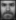
\includegraphics[width=.25\textwidth]{../Images/fa_H/01001_960627_fa}
	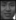
\includegraphics[width=.25\textwidth]{../Images/fa_H/00261_940128_fa}
	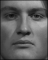
\includegraphics[width=.25\textwidth]{../Images/fa_H/00863_940307_fa}
	\caption{Three high-resolution test images (top) and the training images they were correctly matched against (bottom).}
\end{figure}

\begin{figure}[H]
	\centering
	\includegraphics[width=.25\textwidth]{../Images/fb_L/01001_960627_fb}
	\includegraphics[width=.25\textwidth]{../Images/fb_L/00261_940128_fb}
	\includegraphics[width=.25\textwidth]{../Images/fb_L/00863_940307_fb}\\
	\includegraphics[width=.25\textwidth]{../Images/fa_L/01001_960627_fa}
	\includegraphics[width=.25\textwidth]{../Images/fa_L/00261_940128_fa}
	\includegraphics[width=.25\textwidth]{../Images/fa_L/00863_940307_fa}
	\caption{Three low-resolution test images (top) and the training images they were correctly matched against (bottom).}
\end{figure}

\begin{figure}[H]
	\centering
	\includegraphics[width=.25\textwidth]{../Images/fb_H/00556_940519_fb}
	\includegraphics[width=.25\textwidth]{../Images/fb_H/00212_940128_fb_a}
	\includegraphics[width=.25\textwidth]{../Images/fb_H/00695_941121_fb}\\
	\includegraphics[width=.25\textwidth]{../Images/fa_H/00557_940519_fa}
	\includegraphics[width=.25\textwidth]{../Images/fa_H/00266_940128_fa}
	\includegraphics[width=.25\textwidth]{../Images/fa_H/01005_960627_fa}
	\caption{Three high-resolution test images (top) and the training images they were incorrectly matched against (bottom).}
\end{figure}

\begin{figure}[H]
	\centering
	\includegraphics[width=.25\textwidth]{../Images/fb_L/00770_960530_fb_a}
	\includegraphics[width=.25\textwidth]{../Images/fb_L/00212_940128_fb_a}
	\includegraphics[width=.25\textwidth]{../Images/fb_L/00695_941121_fb}\\
	\includegraphics[width=.25\textwidth]{../Images/fa_L/00494_940519_fa}
	\includegraphics[width=.25\textwidth]{../Images/fa_L/00266_940128_fa}
	\includegraphics[width=.25\textwidth]{../Images/fa_L/00968_960627_fa}
	\caption{Three low-resolution test images (top) and the training images they were incorrectly matched against (bottom).}
\end{figure}

\end{document}